% TEMPLATE for Usenix papers, specifically to meet requirements of
%  USENIX '05
% originally a template for producing IEEE-format articles using LaTeX.
%   written by Matthew Ward, CS Department, Worcester Polytechnic Institute.
% adapted by David Beazley for his excellent SWIG paper in Proceedings,
%   Tcl 96
% turned into a smartass generic template by De Clarke, with thanks to
%   both the above pioneers
% use at your own risk.  Complaints to /dev/null.
% make it two column with no page numbering, default is 10 point

% Munged by Fred Douglis <douglis@research.att.com> 10/97 to separate
% the .sty file from the LaTeX source template, so that people can
% more easily include the .sty file into an existing document.  Also
% changed to more closely follow the style guidelines as represented
% by the Word sample file. 

% Note that since 2010, USENIX does not require endnotes. If you want
% foot of page notes, don't include the endnotes package in the 
% usepackage command, below.

% This version uses the latex2e styles, not the very ancient 2.09 stuff.
\documentclass[letterpaper,twocolumn,10pt]{article}
%\usepackage{usenix,epsfig,endnotes}
\usepackage{usenix}
\usepackage{epsfig}
\usepackage{comment}
%\usepackage{subfigure}
\usepackage[pdftex]{color}
\usepackage{url}
\usepackage{listings}
\usepackage{textcomp}
\usepackage{gnuplot-lua-tikz}
\usepackage{amssymb}
\usepackage{amsmath}
\usepackage{minted}
\usepackage{bm}
\usepackage{paralist}
\usepackage{ulem}
\usepackage{subcaption}
\usepackage{algorithm}
\usepackage{algpseudocode}
\usepackage{graphicx}
\definecolor{lbcolor}{rgb}{0.9,0.9,0.9}

\lstset{
	backgroundcolor=\color{lbcolor},
		tabsize=4,
		rulecolor=,
		language=matlab,
		basicstyle=\scriptsize,
		upquote=true,
		aboveskip={1.5\baselineskip},
		columns=fixed,
		showstringspaces=false,
		extendedchars=true,
		breaklines=true,
		prebreak = \raisebox{0ex}[0ex][0ex]{\ensuremath{\hookleftarrow}},
		frame=single,
		showtabs=false,
		showspaces=false,
		showstringspaces=false,
		identifierstyle=\ttfamily,
		keywordstyle=\color[rgb]{0,0,1},
		commentstyle=\color[rgb]{0.133,0.545,0.133},
		stringstyle=\color[rgb]{0.627,0.126,0.941},
}


\newcommand{\rb}[1]{{\color{red}{\it RB: #1}}}
\newcommand{\dz}[1]{{\color{blue}{\it DZ: #1}}}
\newcommand{\dm}[1]{{\color{green}{\it DM: #1}}}
\newcommand{\hl}[1]{{\color{orange}{#1}}}

\newlength{\saveparindent}
\setlength{\saveparindent}{\parindent}
\newlength{\saveparskip}
\setlength{\saveparskip}{\parskip}

\newenvironment{newenumerate}{%
\begin{list}{({\rm \arabic{ctr}})\hfill}{\usecounter{ctr}\labelwidth=17pt%
\labelsep=6pt \leftmargin=23pt \topsep=.5pt%
\setlength{\listparindent}{\saveparindent}%
\setlength{\parsep}{\saveparskip}%
\setlength{\itemsep}{5pt} }}{\end{list}}

\newenvironment{newitemize}{%
\begin{list}{\hspace{3pt}$\bullet$\hfill}{\labelwidth=12pt%
\labelsep=3pt \leftmargin=15pt \topsep=1pt%
\setlength{\listparindent}{\saveparindent}%
\setlength{\parsep}{\saveparskip}%
\setlength{\itemsep}{1pt}}}{\end{list}}

\begin{document}

%don't want date printed
\date{}

%make title bold and 14 pt font (Latex default is non-bold, 16 pt)
\title{An SSD-based eigensolver for spectral analysis on billion-node graphs}

%for single author (just remove % characters)
%\author{
%{\rm Da Zheng, Randal Burns}\\
%Department of Computer Science \\
%Johns Hopkins University
%\and
%{\rm Joshua Vogelstein}\\
%Institute for Computational Medicine \\
%Department of Biomedical Engineering \\
%Johns Hopkins University
% copy the following lines to add more authors
%\and
%{\rm Alexander S. Szalay}\\
%Department of Physics and Astronomy \\
%Johns Hopkins University
%} % end author

\maketitle

% Use the following at camera-ready time to suppress page numbers.
% Comment it out when you first submit the paper for review.
\thispagestyle{empty}


\subsection*{Abstract}
Many eigensolvers such as ARPACK and Anasazi have been developed to compute
eigenvalues of a large sparse matrix. These eigensolvers are limited by
the capacity of RAM. They run in memory of a single machine for smaller
eigenvalue problems and require the distributed memory for larger problems.

In contrast, we develop an SSD-based eigensolver framework called FlashEigen,
which extends Anasazi eigensolvers to SSDs, to compute eigenvalues of a graph
with hundreds of millions or even billions of vertices in a single machine.
FlashEigen performs sparse matrix multiplication in a semi-external memory
fashion, i.e., we keep the sparse matrix on SSDs and the dense matrix in memory.
%We specifically optimize the
%SpMM implementation for many real-world graphs that have nearly random
%vertex connection and power-law distribution in vertex degree. Due to
%the sparsity of the real-world graphs, the eigensolvers require large
%storage space for the vector subspace.
We store the entire vector subspace on SSDs and reduce I/O to improve
performance through caching the most recent dense matrix.
Our result shows that FlashEigen is able to achieve 40\%-60\% performance
of its in-memory implementation and has performance comparable to the Anasazi
eigensolvers on a machine with 48 CPU cores. Furthermore, it is capable of
scaling to a graph with 3.4 billion vertices and 129 billion edges. It takes
about four hours to compute eight eigenvalues of the billion-node graph using
120 GB memory.

\section{Introduction}
% What problem are you going to solve.
Spectral analysis \cite{} is a fundamental tool for both graph analysis and
other areas of data mining. Essentially, it computes
eigenvalues and eigenvectors of graphs to infer properties of graphs.
spectral clustering \cite{Ng01, Sussman12}, triangle counting \cite{Tsourakakis08}.
Many real-world graphs are massive: Facebook's social network has billions
of vertices and today's web graph is even much larger.

% Why is it hard?

It is computationally expensive to compute all eigenvalues and
eigenvectors of a large matrix. The computation complexity is
$O(n^3)$ on a square matrix \cite{Pan99}, where $n$ is the number of rows
and columns of the matrix.
When the size of a matrix grows to millions or even billions of rows and
columns, it becomes prohibitive to compute all eigenvalues and
eigenvectors.

Numerous algorithms \cite{Lanczos, IRLM, krylovschur, Arbenz05} have been
developed to compute a small number of eigenpairs.
The current popular eigensolver packages such as ARPACK \cite{arpack}
and Anasazi \cite{anasazi} have state-of-art eigensolvers
capable of computing a few eigenvalues with certain properties such as
the eigenvalues of the largest or smallest magnitude. All of these eigensolvers
perform a sequence of sparse matrix multiplication to construct and update
a vector subspace $S \in \mathbb{R}^{n \times m}$, where $n$ is the size of
the eigenproblem and $m$ is the subspace size \cite{Arbenz05}. In addition,
they perform multiple matrix operations on very large dense matrices that
stores the vector subspace. When computing eigenpairs of a graph
at the billion scale, neither the sparse matrix that represents a graph nor
the dense matrices can be stored in RAM in a single machine.

%How have others addressed the problem?
Therefore, large-scale eigendecomposition is generally solved in a large cluster
or a supercomputer \cite{anasazi, slepc}, where the aggregated memory is
sufficient to store the sparse matrix and the dense matrices for
the subspace. However, many real-world graphs have the power-law distribution
in vertex degree and near-random vertex connection. Sparse matrix multiplication
on such a graph leads to significant network communication. As such, it requires
fast network to achieve overall performance. However, a supercomputer or a large
cluster with fast network communication is not accessible to many people.

%What is the nature of your solution?

We build FlashEigen, an external-memory eigensolver, to solve a large eigenproblem
with SSDs in a single machine. 
%Today's SSDs or SSD arrays
%are capable of delivering over a million random IOPS or multiple GB/s of
%sequential I/O \cite{safs}. Given such I/O performance, it is possible to
%achieve nearly in-memory performance for large-scale graph analysis using SSDs
%\cite{flashgraph}. In this paper, we focus on utilizing SSDs for
%spectral graph analysis as well as general linear algebra.
Instead of developing a new eigensolver from scratch, we leverage
the Anasazi framework and implement SSD-based matrix operations
for the framework. FlashEigen is specifically optimized for the Block
Krylov-Schur \cite{krylovschur} eigensolver because it is the fastest and
generates the least I/O among the Anasazi eigensolvers when computing
eigenvalues of many power-law graphs. The Anasazi eigensolvers implement
a block extension, which enables the eigensolvers to update multiple vectors
in the subspace in each iteration to increase computation density and amortize
I/O overhead. As a result, the eigensolvers require sparse matrix dense matrix
multiplication (SpMM). We perform SpMM in a semi-external memory fashion, i.e.,
the sparse matrix on SSDs and the input dense matrix in memory. Given a graph
with hundreds of millions of vertices or even billions of vertices,
the vector subspace constructed by the eigensolvers requires very large storage
size, usually much larger than the sparse matrix. Therefore, FlashEigen stores
the entire vector subspace on SSDs.

Although SSDs can deliver high IOPS and sequential I/O throughput, we have
to overcome many technical challenges to construct an external-memory
eigensolver with performance comparable to in-memory eigensolvers.
SSDs are an order of magnitude slower than DRAM in throughput. Furthermore,
SSDs wear out after we write data to them. For example, some enterprise SSDs
\cite{} only allows one DWPD (diskful writes per day).

We specifically optimize semi-external memory sparse matrix dense matrix
multiplication for many real-world graphs that have nearly random vertex
connection and power-law distribution in vertex degree. We deploy a series of
optimizations for both in-memory computation and I/O.
NUMA, blocking, vectorization, compress sparse matrix, split the dense matrix
so that we can still use semi-external memory SpMM.

We further deploy optimizations on dense matrix operations to reduce I/O and
fully utilize the I/O bandwidth of the SSDs.
To reduce I/O and the amount of data written to SSDs, we use lazy evaluation.
caching if the dense matrix is very narrow.

% Why is it new/different/special?

% What are it's key features?

Out result shows that the SSD-based KrylovSchur eigensolver is able to achieve
about 50\% performance of its in-memory implementation and the original
KrylovSchur in the Anasazi framework on a machine with 48 CPU cores for
computing various numbers of eigenvalues. Furthermore, it is
capable of scaling to a graph with 3.4 billion vertices and 129 billion edges.
It takes xxx hours to compute xxx singular values of the billion-node direct graph
and use xxx GB memory.


\section{Related Work}
Anasazi \cite{anasazi} is an eigensolver framework in the Trilinos project
\cite{trilinos}. This framework implements block extension of multiple
eigensolver algorithms
such as Block Krylov-Schur method \cite{krylovschur}, Block Davidson method
\cite{Arbenz05} and LOBPCG \cite{Arbenz05}. This is a very flexible framework
that allows users to redefine sparse matrix dense matrix multiplication and
dense matrix operations. By default, Anasazi uses the matrix implementations
in Trilinos that run in the distributed memory.

Arpack \cite{arpack} is another state-of-art eigensolver commonly used by
multiple numeric computation frameworks such as Matlab. This eigensolver
implements the implicitly restarted arnoldi method \cite{IRAM}. Arpack
only allows users to redefine sparse matrix vector multiplication.
Its dense matrix operations by default run in serial.

Sparse matrix vector multiplication (SpMV) and sparse matrix dense matrix
multiplication (SpMM) are an important operation in numeric computation and
are well studied in the literature. For example, Williams et. al
\cite{Williams07} described multiple optimizations for sparse matrix
vector multiplication in multicore architecture. Yoo et. al \cite{Yoo11}
and Boman et. al \cite{Boman2013} optimized SpMV for large scale-free graphs
using 2D graph partitioning. Sparse matrix multiple vector multiplication
\cite{Aktulga14}

FlashGraph \cite{flashgraph} is a general graph analysis framework. It performs
graph algorithms in a semi-external memory fashion \cite{sem}, i.e., it keeps
vertex state in memory and edge lists on SSDs. It is specifically optimized for
graph algorithms that has a fraction of vertices running in each iteration.
This design prevents FlashGraph from performing some optimizations for sparse
matrix multiplication as shown in this paper.

HEIGEN \cite{Kang11} is an eigensolver implemented with MapReduce \cite{mapreduce}
to compute eigenpairs for spectral graph analysis. HEIGEN implements a basic
Lanczos algorithm
\cite{Lanczos} with selective orthogonalization from scratch. In contrast, our
approach extends the state-of-art implementations to SSDs. By integrating many
SSDs to a single machine, our approach can compete with a cluster.

Zhou et al. \cite{Zhou12} implemented an LOBPCG \cite{Arbenz05} eigensolver in
an SSD cluster. Their implementation targets nuclear many-body Hamiltonian
matrices, which are much denser and have smaller dimensions than many sparse
graphs. Therefore, their solution stores dense matrices in the subspace in RAM.
Their solution also focus on optimizations in the distributed
environment. In contrast, we have to store dense matrices in the subspace
on SSDs due to the large number of vertices in our target graphs. We focus
on external-memory optimizations in a single machine.

Eigendecomposition
is a well studied problem and many more advanced algorithms have been proposed
in the past decades. These algorithms are able to compute eigenpairs with
different properties such as the largest-magnitude or the smallest-magnitude
eigenvalues.


\section{Design}
FlashEigen is an external-memory eigensolver optimized for any fast I/O devices
such as a large SSD array to compute eigenvalues of sparse graphs. It takes
advantage of the flexible programming interface of the Anasazi framework and
focuses on optimizing sparse matrix dense matrix multiplication and dense
matrix operations on SSDs.

\subsection{Eigensolver algorithm}

%\begin{figure}
%\centering
%\includegraphics[scale=0.35]{./SpMM.pdf}
%\vspace{-5pt}
%\caption{}
%\vspace{-5pt}
%\label{SpMM}
%\end{figure}

\begin{algorithm}
	\begin{algorithmic}[1]
		\For{i = 0, 1, ..., until convergence}
		\State (1) Update the subspace $S \in \mathbb{R}^{n \times m}$,
		\State (2) Solve the projected eigenproblem $S^TASy = S^TSy\theta$.
		\State (3) Compute the residual: $r = Kx - x\theta$, where
		\State\hspace{\algorithmicindent} $x = Sy$ (Ritz vector), $\theta = \rho(x)$ (Ritz value).
		\State (4) Test the convergence of a Ritz pair $(x, \rho(x))$.
		\EndFor
	\end{algorithmic}
	\caption{Pseudo code of a generic eigenvalue algorithm that compute eigenvalues
	of a square matrix $A$ with $n$ rows and columns.}
	\label{eigencode}
\end{algorithm}

The state-of-art eigenvalue algorithms compute eigenvalues with iterative
methods. Figure \ref{eigencode} shows the general steps used by the eigenvalue
algorithms.
Step (1) constructs a vector subspace $S \in \mathbb{R}^{n \times m}$, where
$n$ is the number of rows and columns of a sparse matrix and $m$ is the number
of vectors in the subspace. When computing eigenvalues of a sparse graph,
two key operations in this step are sparse matrix multiplication to construct
the subspace and reorthogonalization to correct float-point rounding errors.
A block extenion of an eigensolver updates multiple vectors in the subspace
in a single step, which leads to sparse matrix dense matrix multiplication.
Step (2) projects the large sparse matrix to a much smaller matrix with only
$m$ rows and $m$ columns, which can be solved by other eigensolvers such as
the one in LAPACK \cite{lapack}. Step (3) projects the solution of the small
eigenvalue problem back to the original eigenvalue problem. Step (4) tests
whether the projected solution fulfills the precision requirement given by
users. If not, the algorithm may adjust the vector subspace, jump back to
step (1) and continue the process.

\subsection{The architecture of FlashEigen}

We build FlashEigen on top of SAFS, a user-space filesystem, to fully utilize
the I/O throughput of a large SSD array. The architecture of FlashEigen is shown
in Figure \ref{arch}. FlashEigen has two main components that process sparse
matrices and dense matrices respectively. It stores data of sparse matrices
and dense matrices
in SAFS and implements matrix operations required by the Anasazi eigensolvers.
As such, the Anasazi eigensolvers can access data from SSDs.

\begin{figure}
\centering
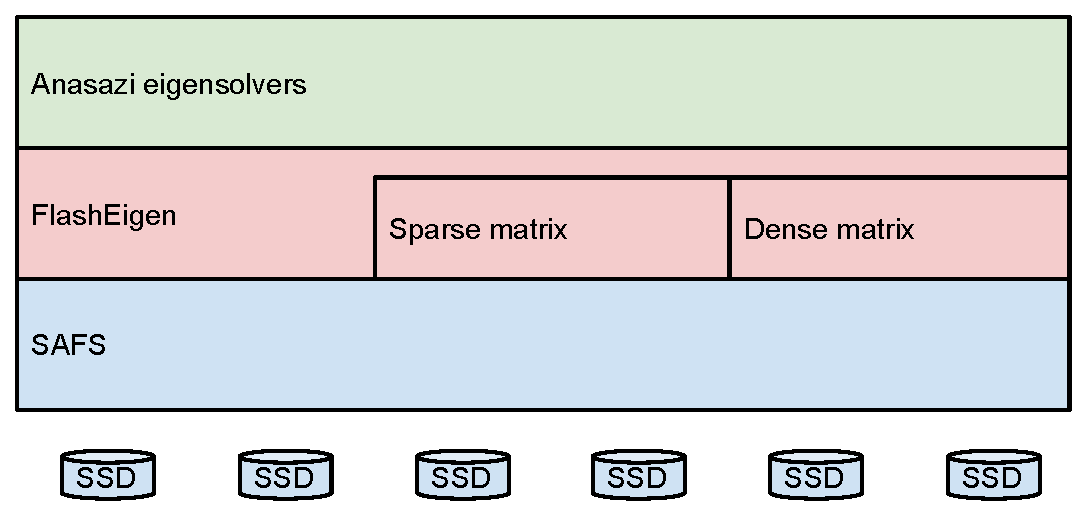
\includegraphics[scale=0.4]{./architecture.pdf}
\vspace{-5pt}
\caption{The architecture of FlashEigen.}
\vspace{-5pt}
\label{arch}
\end{figure}

\subsection{SAFS}

SAFS \cite{safs} is a user-space filesystem for a high-speed SSD array in
a NUMA machine. It is implemented as a library and runs in the address space
of its application. It is deployed on top of the Linux native filesystem.
SAFS was originally designed for optimizing small I/O accesses. However,
sparse matrix multiplication and dense matrix operations
generate much fewer but much larger I/O. Therefore, we provide additional
optimizations to maximize sequential I/O throughput from a large SSD array.

The original SAFS has a dedicated I/O thread for each SSD. The I/O thread
accesses the SSD exclusively to avoid lock contention in the Linux kernel.
Application threads have to send I/O requests to one of the I/O threads
with message passing when accessing data from SSDs. It is necessary to have
one I/O thread for
an SSD when applications issue many small I/O accesses because processing
a large number of I/O accesses consumes a significant number of CPU cycles.
However, when the workload only has large I/O requests, each I/O request takes
much longer time to complete. As a result, the I/O threads are constantly put
into sleep while waiting for I/O and each I/O completion may suffer from
the latency of a thread context switch.

The latency of a thread context switch becomes noticeable on a high-speed SSD
array under a sequential I/O workload and it becomes critical to avoid thread
context switch to gain I/O performance. Therefore, instead of having an I/O
thread for each SSD, we use only a single I/O thread for each NUMA node, which
is responsible for all of the SSDs connected to the NUMA node. As such, an I/O
thread processes many more I/O requests to amortize the latency of a context
switch. Similarly, application threads communicate with I/O threads through
message passing when issuing I/O requests. If the computation in application
threads did not saturate CPU, SAFS would put the application threads into
sleep while they were waiting for I/O. This results in many thread context
switches and underutilization of both CPU and SSDs. To saturate I/O,
an application thread issues asynchronous I/O and poll for I/O to avoid thread
context switches after completing all computation available to it.

To better support access to many relatively small files simultaneously, SAFS
stripes data in a file across SSDs with a different striping order for each file.
This strategy stores data from multiple files evenly across SSDs and improves
I/O utialization. Due to the sequential I/O workload, FlashEigen stripes data
across SSDs with a large block size, in the order of multiple
megabytes, to increase I/O throughput and potentially reduce write amplification
on SSDs \cite{}. Such a large block size may cause storage skew for small files
on a large SSD array if every file stripes data in the same order. Using
the same striping order for all files may also cause skew in I/O access.
Therefore, SAFS generates a random striping order for each file to evenly
distribute I/O among SSDs when a file is created. SAFS stores the striping
order with the file for future data retrieval.

\subsection{Sparse matrix multiplication} \label{spmm}
Sparse matrix multiplication is a computationally expensive
operation in an eigensolver due to random memory access. Sparse matrix vector
multiplication (SpMV) is usually limited by the random memory performance of
DRAM. Sparse matrix dense matrix multiplication (SpMM) increases data locality
and improve overall performance of an eigensolver. Therefore, a block extension
of an eigensolver is preferred.

To scale sparse matrix multiplication to a sparse graph with billions of vertices,
we perform sparse matrix multiplication in semi-external memory (SEM). That is,
we keep the vectors or dense matrices in memory and the sparse
matrix on SSDs. This strategy enables nearly in-memory performance while achieving
the scalability in proportion to the ratio of edges to vertices in a graph.

\subsubsection{The sparse matrix format}
The state-of-art numeric libraries store a sparse matrix in compressed row storage
(CSR) or compressed column storage (CSC) format. However, these formats incur
many CPU cache misses in sparse matrix multiplication on many real-world graphs
due to their nearly random vertex connection. They also require a relatively
large storage size. For a graph with billions of edges, we have to use eight
bytes to store the row and column indices. For semi-external memory sparse
matrix multiplication, SSDs may become the bottleneck if a sparse matrix has
a large storage size.
Therefore, we need to use an alternative format for sparse matrices to increase
CPU cache hits and reduce the amount of data read from SSDs.

\begin{figure}
\centering
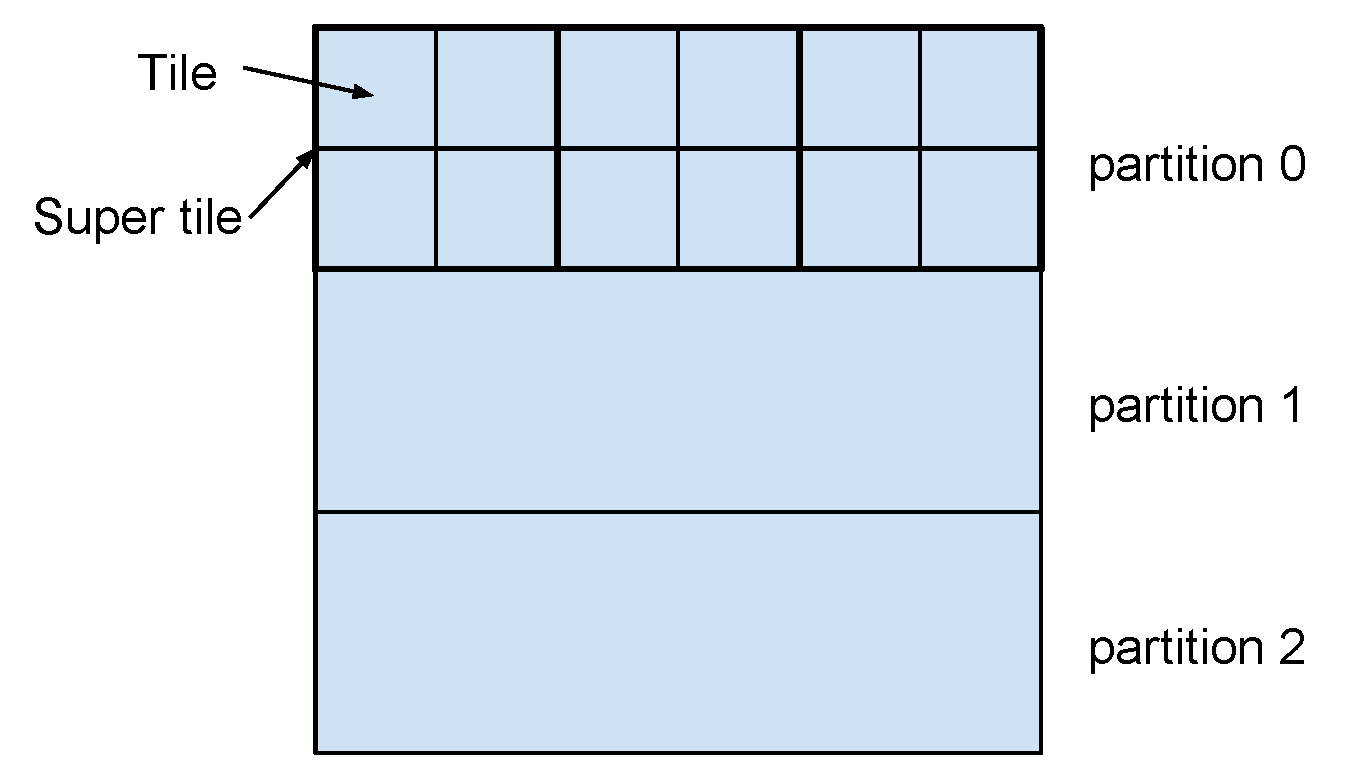
\includegraphics[scale=0.3]{./sparse_mat.pdf}
\vspace{-5pt}
\caption{}
\vspace{-5pt}
\label{sparse_mat}
\end{figure}

To increase CPU cache hits, we deploy cache blocking \cite{Im04} and store
non-zero entries of a sparse matrix in tiles (Figure \ref{sparse_mat}).
When a tile is small, the rows from the input and output dense matrices
involved in the multiplication with the tile are always kept in the CPU cache
during the multiplication. The optimal tile size should fill the CPU cache
with the rows of the dense matrices involved in the multiplication with
the tile and is affected by the number of columns of the dense matrices,
which are chosen by users. Instead of generating a sparse matrix with
different tile sizes optimized for different numbers of columns in the dense
matrices, we use a relatively small tile size and rely on the runtime system
to optimize for different numbers of columns (in section \ref{sec:exec}).
In the semi-external memory, we expect that the dense matrices do not
have more than eight columns in sparse matrix multiplication. Therefore, we
use the tile size of $16K \times 16K$ by default to balance the matrix storage
size and the adaptibility to different numbers of columns.

\begin{figure}
\centering
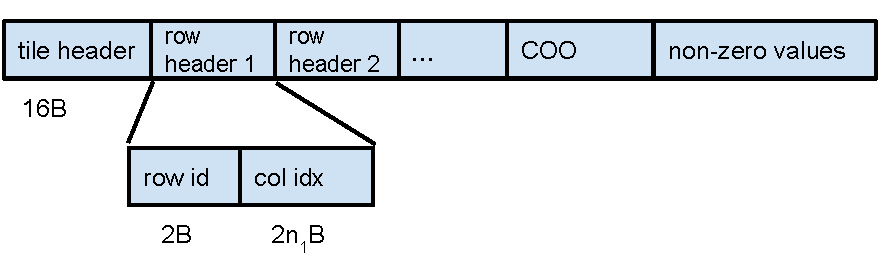
\includegraphics[scale=0.5]{./tile_format.pdf}
\vspace{-5pt}
\caption{The storage format of a tile in a sparse matrix.}
\vspace{-5pt}
\label{tile_format}
\end{figure}

To reduce the overall storage size of a sparse matrix, we use a compact format
to store non-zero entries in a tile. In very sparse matrices such as
many real-world graphs, many rows in a tile do not have any non-zero entries.
The CSR (CSC) format requires an entry for each row (column) in the row
(column) index. Therefore, the CSR or CSC format waste space when storing elements
in a tile. Instead, we only keep data for rows with non-zero entries in a tile
shown in Figure \ref{tile_format} and refer to this format as SCSR (Super
Compressed Row Storage). This format maintains a row header for each non-empty
row. A row header has an identifier to indicate the row number, followed by
column indices. 
The most significant bit of the identifier is always set to 1, while the most
significant bit of a column index entry is always set to 0. As such, we can easily
distinguish a row identifier from a column index entry and determine the end
of a row. Thanks to the small size of a tile, we use two bytes to further store a row
number and a column index entry to reduce the storage size. Since the most
significant bit is used to indicate the beginning of a row, this format allows
a maximum tile size of $32K \times 32K$.

For many real-world graphs, many rows in a tile have only one non-zero entries,
thanks to their sparsity and nearly random vertex connection. Storing these
single-entry rows in the SCSR format results in many conditional jump CPU
instructions in sparse matrix multiplication.
In contrast, the coordinate format (COO) is more suitable for storing these
single-entry rows. It does not increase the storage size but significantly
reduces the number of conditional jump instructions when we iterate
them. As a result, we hybrid SCSR and COO to store non-zero entries in a tile
with COO stored behind the row headers of SCSR. All non-zero entries are
stored together at the end of a tile.

We organize tiles in a sparse matrix in tile rows and maintain a matrix index
for them. Each entry of the index stores the location of a tile row on SSDs
to facilitate random access
to tile rows. This is useful for parallelizing sparse matrix multiplication.
Because a tile contains thousands of rows, the matrix index requires a very
small storage size even for a billion-node graph. We keep the entire index
in memory during sparse matrix multiplication.

\subsubsection{The dense matrix format for SpMM} \label{numa_mat}
Dense matrices in sparse matrix multiplication are tall-and-skinny matrices
with millions or even billions of rows but only several columns. We organize
elements of the dense matrices in row-major order to increase data locallity,
as shown in Figure \ref{dense_mat} (a).

For a non-uniform memory architecture (NUMA), we partition the input dense matrix
horizontally and store partitions evenly across NUMA nodes to fully utilize
the bandwidth of memory and inter-processor links in sparse matrix
multiplication. The NUMA architecture is commonly used in today's multi-processor
servers, where each processor connects to its own memory banks. It is essential
to fully utilize the bandwidth of memory and inter-processor links to achieve
performance. As shown in Figure \ref{dense_mat} (a), we assign multiple
contiguous rows in a row interval to a partition, which is assigned to a NUMA
node. A row interval always has $2^i$ rows for efficiently locating a row
with bit operations. The row interval size is also multiple of the tile size of
a sparse matrix so that multiplication on a tile only needs to access rows
from a single row interval.

\begin{figure}
\centering
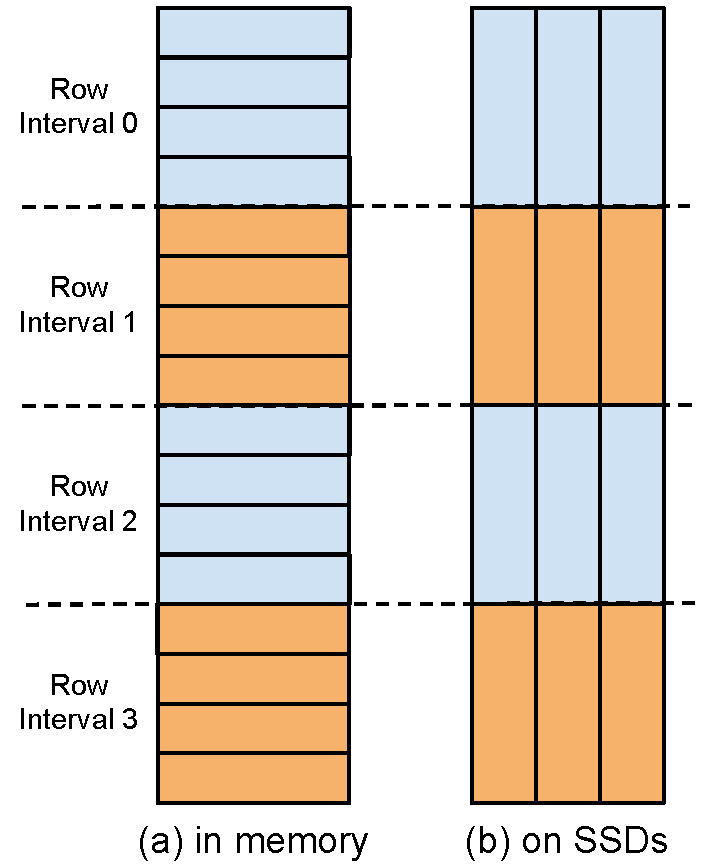
\includegraphics[scale=0.4]{./dense_matrix.pdf}
\vspace{-5pt}
\caption{The data layout of tall-and-skinny dense matrices. A tall-and-skinny
dense matrix is partitioned horizontally into many row intervals.
(a) For an in-memory matrix, row intervals are stored across NUMA nodes and
elements are stored in row-major order; (b) for an SSD-based matrix, elements
inside a row interval are stored in column-major order.}
\vspace{-5pt}
\label{dense_mat}
\end{figure}

\subsubsection{Execution of sparse matrix multiplication} \label{sec:exec}
We perform sparse matrix dense matrix multiplication in semi-external memory
and optimize it for different numbers of columns in the dense matrices.

We partition a sparse matrix horizontally for parallelization and assign multiple
contiguous tile rows to the same partition (Figure \ref{sparse_mat}).
The number of tile rows assigned to a partition is determined at runtime
based on the number of columns in the input dense matrix. A thread reads
a partition of the sparse matrix asynchronously from SSDs. Once a partition
is ready in memory, the worker thread multiplies the partition with the input
dense matrix. The thread processes one tile at a time and stores
the intermediate result in a buffer allocated in the local memory to reduce
remote memory access. To reduce memory consumption,
we write the portion of the output dense matrix to SSDs immediately whenever
it is generated. \dz{Implement this.}

To better utilize CPU cache, we process tiles of a partition in
\textit{super tile}s (Figure \ref{sparse_mat}). The tile size of a sparse
matrix is specified when the sparse matrix image is created and is relatively
small to handle different numbers of columns in the dense matrices.
A \textit{super tile} is composed of tiles from multiple tile rows and its
size is determined at runtime by three factors: the number of columns
in the dense matrices, the CPU cache size and the number of threads that
share the CPU cache. An optimal size for a \textit{super tile} fills
the CPU cache with the rows from the dense matrices involved in
the computation with the \textit{super tile}.

Load balancing also plays a key role in sparse matrix multiplication on
many real-world graphs due to their power-law distribution in vertex degree.
In FlashEigen, a worker thread first processes partitions originally assigned
to the thread. When a worker thread finishes
all of its own partitions, it steals partitions that have not been processed
from other worker threads.

In spite of nearly random edge connection in a real-world graph,
there exists regularity that allows vectorization to improve performance
in sparse matrix dense matrix multiplication. For each non-zero entry, we
need to multiply it with the corresponding row from the input dense matrix
and add the result to the corresponding row in the output dense matrix.
These operations can be accomplished by the vector CPU instructions such as
AVX \cite{avx}. The current implementation relies on GCC's auto-vectorization
to translate the C code to the vector CPU instructions by predefining the matrix
width in the code.

\subsection{Dense matrix operations}
The vector subspace required by an eigensolver is massive when the eigensolver
computes eigenvalues of a billion-node graph or computes many eigenvalues
of a multi-million-node graph. The number of vectors in the subspace
increases with the number of required eigenvalues. Furthermore, a larger
number of vectors in the subspace improves the convergence rate of an eigensolver. 
It is often that the storage size required by the subspace is larger than
the sparse matrix for eigendecomposition on many real-world graphs. Therefore,
FlashEigen stores these vectors on SSDs.

The Anasazi framework provides a set of programming interface to expose
the vectors in the subspace to users as dense matrices and allow users to
redefine the dense matrices and the operations on them. FlashEigen implements
the programming interface and stores the vectors of the subspace on SSDs.
The Anasazi eigensolvers update multiple vectors of the subspace in an iteration
due to the block extension, so FlashEigen stores multiple vectors in a dense
matrix physically and the number of vectors in a matrix is determined by
the block size of a block eigensolver. This design also helps garbage
collection in lazy evaluation (section \ref{sec:lazy_eval}).
As such, the subspace is composed of multiple tall-and-skinny dense matrices.

\begin{table}
	\begin{center}
		\small
		\begin{tabular}{|c|c|c|c|c|}
			\hline
			& operation & customized output \\
			\hline
			op1 & $CC \leftarrow \alpha \times AA \times B + \beta \times CC$ & yes \\
			\hline
			op2 & $BB \leftarrow AA \times diag(vec)$ & yes \\
			\hline
			op3 & $A \leftarrow \alpha \times t(AA) \times BB$ & no \\
			\hline
			op4 & $CC \leftarrow \alpha \times AA + \beta \times BB$ & yes \\
			\hline
			op5 & $BB \leftarrow \alpha \times AA$ & yes \\
			\hline
			op6 & $vec \leftarrow norm\_col(AA)$ & no \\
			\hline
			op7 & $BB \leftarrow AA[,idxs]$ & yes \\
			\hline
			op8 & $AA[,idxs] \leftarrow BB$ & yes \\
			\hline
			op9 & $AA \leftarrow conv\_layout(BB)$ & yes \\
			\hline
		\end{tabular}
		\normalsize
	\end{center}
	\caption{The dense matrix operations required by the Anasazi eigensolvers.
		$XX$ represents a tall dense matrix, $X$ represents a small dense matrix,
	$\alpha$ and $\beta$ represents scalar variables.}
	\label{anasazi_ops}
\end{table}

FlashEigen requires a set of dense matrix operations shown in Table
\ref{anasazi_ops}. $op1-8$ are the operations required by the Anasazi
framework. The most computationally expensive operations are the two
matrix multiplication operations: $op1$ and $op3$, mainly used for
reorthogonalization to fix float-point rounding errors. The eigensolvers
use $op7$ and $op8$ to access individual columns of a dense matrix,
so we store the dense matrices in column major by default.
However, the sparse matrix dense matrix multiplication described in section
\ref{spmm} requires a row-major dense matrix to increase data locality.
Thus, FlashEigen adds another operation $op9$ to convert data layout
in dense matrices, which converts a column-major matrix to a row-major
matrix when it is passed to the SpMM operation.

It is challenging to achieve the performance of external-memory dense matrix
operations comparable to their in-memory counterparts. Unlike sparse matrix
multiplication, these dense matrix operations are less memory intensive.
Even though SSDs are fast, their sequential I/O performance is still an order
of magnitude slower than RAM.
Furthermore, SSDs wears out after a certain amount of write \cite{}.
Even enterprise SSDs \cite{} only allows a small number of DWPD
(diskful writes per day). Therefore, FlashEigen optimizes dense matrix operations
with three goals: \textit{(i)} maximizing I/O throughput from SSDs,
\textit{(ii)} minimizing the amount of data read from SSDs,
\textit{(iii)} reducing SSD wearout.

%\begin{figure}
%	\begin{center}
%		\footnotesize
%		\vspace{-15pt}
%		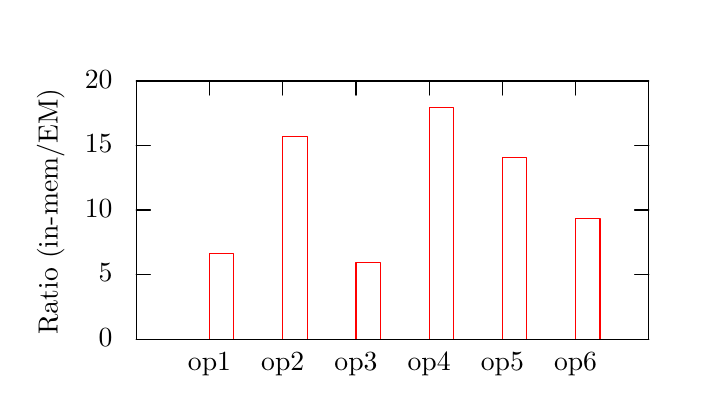
\begin{tikzpicture}[gnuplot]
%% generated with GNUPLOT 4.6p4 (Lua 5.1; terminal rev. 99, script rev. 100)
%% Thu 16 Jul 2015 09:41:54 AM EDT
\path (0.000,0.000) rectangle (8.382,4.572);
\gpcolor{color=gp lt color border}
\gpsetlinetype{gp lt border}
\gpsetlinewidth{1.00}
\draw[gp path] (1.320,0.616)--(1.500,0.616);
\draw[gp path] (7.829,0.616)--(7.649,0.616);
\node[gp node right] at (1.136,0.616) { 0};
\draw[gp path] (1.320,1.436)--(1.500,1.436);
\draw[gp path] (7.829,1.436)--(7.649,1.436);
\node[gp node right] at (1.136,1.436) { 5};
\draw[gp path] (1.320,2.256)--(1.500,2.256);
\draw[gp path] (7.829,2.256)--(7.649,2.256);
\node[gp node right] at (1.136,2.256) { 10};
\draw[gp path] (1.320,3.075)--(1.500,3.075);
\draw[gp path] (7.829,3.075)--(7.649,3.075);
\node[gp node right] at (1.136,3.075) { 15};
\draw[gp path] (1.320,3.895)--(1.500,3.895);
\draw[gp path] (7.829,3.895)--(7.649,3.895);
\node[gp node right] at (1.136,3.895) { 20};
\draw[gp path] (2.250,0.616)--(2.250,0.796);
\draw[gp path] (2.250,3.895)--(2.250,3.715);
\node[gp node center] at (2.250,0.308) {op1};
\draw[gp path] (3.180,0.616)--(3.180,0.796);
\draw[gp path] (3.180,3.895)--(3.180,3.715);
\node[gp node center] at (3.180,0.308) {op2};
\draw[gp path] (4.110,0.616)--(4.110,0.796);
\draw[gp path] (4.110,3.895)--(4.110,3.715);
\node[gp node center] at (4.110,0.308) {op3};
\draw[gp path] (5.039,0.616)--(5.039,0.796);
\draw[gp path] (5.039,3.895)--(5.039,3.715);
\node[gp node center] at (5.039,0.308) {op4};
\draw[gp path] (5.969,0.616)--(5.969,0.796);
\draw[gp path] (5.969,3.895)--(5.969,3.715);
\node[gp node center] at (5.969,0.308) {op5};
\draw[gp path] (6.899,0.616)--(6.899,0.796);
\draw[gp path] (6.899,3.895)--(6.899,3.715);
\node[gp node center] at (6.899,0.308) {op6};
\draw[gp path] (1.320,3.895)--(1.320,0.616)--(7.829,0.616)--(7.829,3.895)--cycle;
\node[gp node center,rotate=-270] at (0.246,2.255) {Ratio (in-mem/EM)};
\def\gpfillpath{(2.250,0.616)--(2.561,0.616)--(2.561,1.709)--(2.250,1.709)--cycle}
\gpfill{color=gpbgfillcolor} \gpfillpath;
\gpfill{color=gp lt color 0,gp pattern 0,pattern color=.} \gpfillpath;
\gpcolor{color=gp lt color 0}
\gpsetlinetype{gp lt plot 0}
\draw[gp path] (2.250,0.616)--(2.250,1.708)--(2.560,1.708)--(2.560,0.616)--cycle;
\def\gpfillpath{(3.180,0.616)--(3.491,0.616)--(3.491,3.193)--(3.180,3.193)--cycle}
\gpfill{color=gpbgfillcolor} \gpfillpath;
\gpfill{color=gp lt color 0,gp pattern 0,pattern color=.} \gpfillpath;
\draw[gp path] (3.180,0.616)--(3.180,3.192)--(3.490,3.192)--(3.490,0.616)--cycle;
\def\gpfillpath{(4.110,0.616)--(4.421,0.616)--(4.421,1.593)--(4.110,1.593)--cycle}
\gpfill{color=gpbgfillcolor} \gpfillpath;
\gpfill{color=gp lt color 0,gp pattern 0,pattern color=.} \gpfillpath;
\draw[gp path] (4.110,0.616)--(4.110,1.592)--(4.420,1.592)--(4.420,0.616)--cycle;
\def\gpfillpath{(5.039,0.616)--(5.350,0.616)--(5.350,3.555)--(5.039,3.555)--cycle}
\gpfill{color=gpbgfillcolor} \gpfillpath;
\gpfill{color=gp lt color 0,gp pattern 0,pattern color=.} \gpfillpath;
\draw[gp path] (5.039,0.616)--(5.039,3.554)--(5.349,3.554)--(5.349,0.616)--cycle;
\def\gpfillpath{(5.969,0.616)--(6.280,0.616)--(6.280,2.927)--(5.969,2.927)--cycle}
\gpfill{color=gpbgfillcolor} \gpfillpath;
\gpfill{color=gp lt color 0,gp pattern 0,pattern color=.} \gpfillpath;
\draw[gp path] (5.969,0.616)--(5.969,2.926)--(6.279,2.926)--(6.279,0.616)--cycle;
\def\gpfillpath{(6.899,0.616)--(7.210,0.616)--(7.210,2.152)--(6.899,2.152)--cycle}
\gpfill{color=gpbgfillcolor} \gpfillpath;
\gpfill{color=gp lt color 0,gp pattern 0,pattern color=.} \gpfillpath;
\draw[gp path] (6.899,0.616)--(6.899,2.151)--(7.209,2.151)--(7.209,0.616)--cycle;
\gpcolor{color=gp lt color border}
\gpsetlinetype{gp lt border}
\draw[gp path] (1.320,3.895)--(1.320,0.616)--(7.829,0.616)--(7.829,3.895)--cycle;
%% coordinates of the plot area
\gpdefrectangularnode{gp plot 1}{\pgfpoint{1.320cm}{0.616cm}}{\pgfpoint{7.829cm}{3.895cm}}
\end{tikzpicture}
%% gnuplot variables

%		\vspace{-15pt}
%		\caption{The relative performance of external-memory matrix operations
%			on a dense matrix with 200M rows and 16 columns on an array of 24
%		SSDs.}
%		\label{perf:mat_ops}
%	\end{center}
%\end{figure}

\subsubsection{Parallelization and external memory access} \label{par_em}
We partition the tall-and-skinny matrices horizontally for parallelization
and external-memory access. Figure \ref{dense_mat} (b) illustrates the format
of an external-memory tall-and-skinny matrix. Like a NUMA dense matrix in
Figure \ref{dense_mat} (a),
an external-memory matrix is divided into multiple row intervals and data
in a row interval is stored contiguously. Unlike a NUMA dense matrix, elements
in a row interval of an external-memory matrix are stored in column-major order
for easily accessing individual columns. The size of a row interval is chosen
according to the number of columns in the matrix to generate large I/O requests,
in the order of megabytes.

Once data in a row interval is loaded to memory, we further partition it to
smaller row intervals so that data
in the sub-row interval fits in CPU cache. \dz{TODO: The size of the sub row
interval should also adapt to the matrix width.} This optimization significantly
increase CPU cache hits in a sequence of dense matrix operations constructed in
the lazy evaluation (Section \ref{sec:lazy_eval}).

To parallelize a matrix operation, we assign one row interval at a time to
a worker thread. When a worker thread gets a row interval, it owns the row
interval and is responsible for accessing the data in the row interval from
all of the tall-and-skinny matrices and performing computation on them.
When processing a row interval, a worker thread does not need to access data
from another row interval on SSDs.
%(Figure \ref{fig:mat_par}).
Majority of the operations in Table \ref{anasazi_ops} output tall-and-skinny
matricies whose rows only depend on the same rows from the input matrices.
For these operations, the computation and data access to the tall-and-skinny
matrices are completely independant between row intervals. One of the exceptions is
$op3$, which outputs a small matrix. However, this operation can be split into
two sub-operations: the first one performs computation on data in the same row
interval from all of the input matrices and output a small matrix and the computation
is completely independant between row intervals; the second one sums all of
the small matrices and outputs a single small matrix. The first sub-operation
has most of computation in $op3$ and requires external-memory data access,
so we parallelize it in the same fashion as other operations.
%This is illustrated in Figure \ref{fig:mat_par}.
$op6$ can be evaluated in a similar fashion to $op3$. Therefore, all matrix
operations in Table \ref{anasazi_ops} can be parallelized in the same fashion.

%\dz{a large write is required to achieve persistent write performance and
%wearout?}
%We maintain a global work queue of row intervals and dispatch one row interval
%to a thread at a time. This strategy allows worker threads to process row
%intervals close to each other, which helps to accumulate very large writes to SSDs.

\begin{figure}
\centering
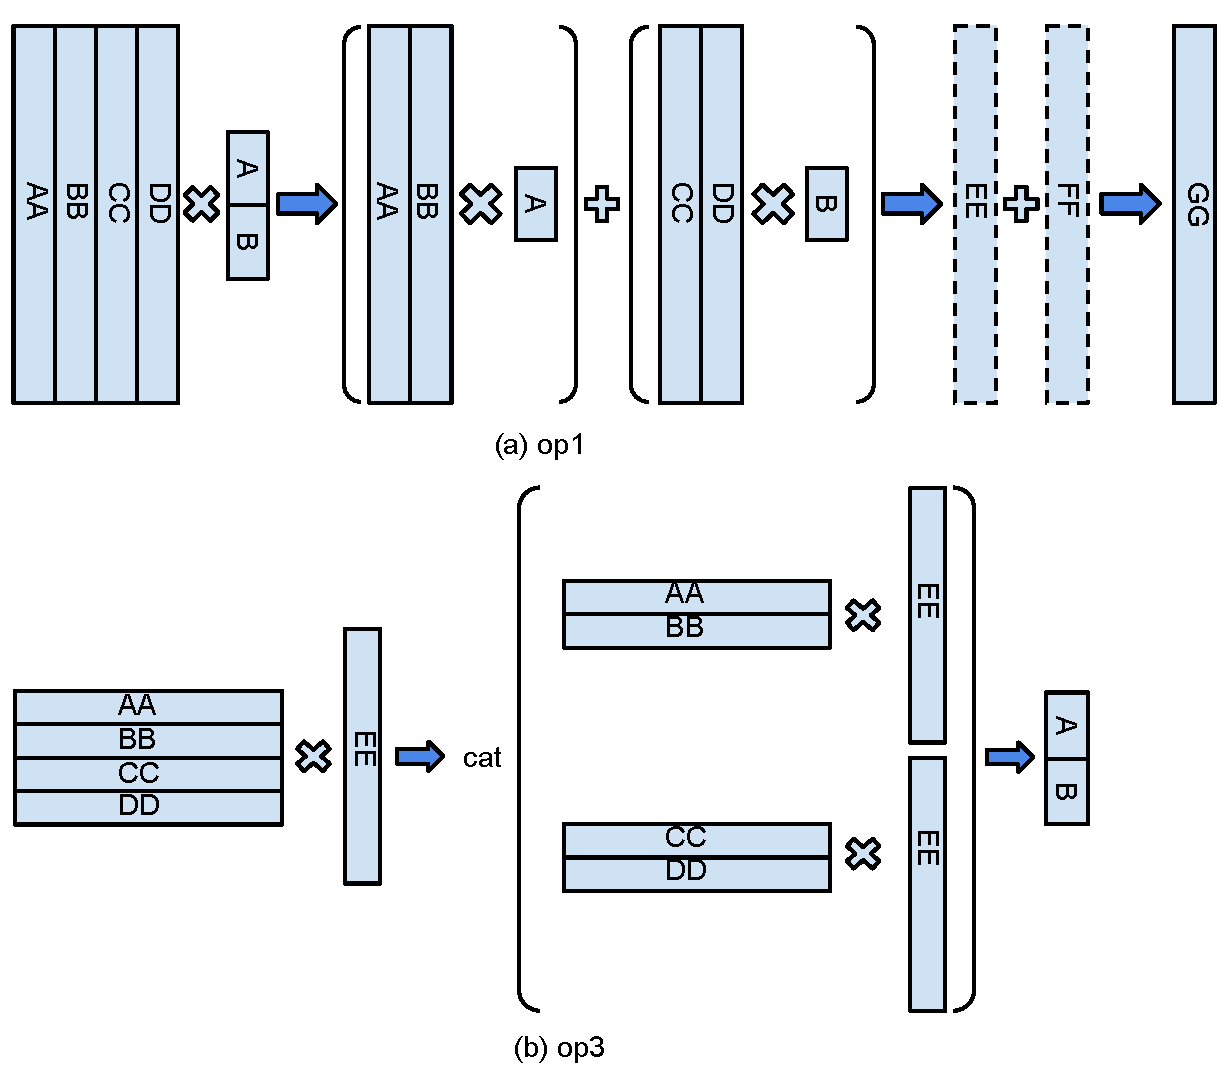
\includegraphics[scale=0.4]{./mat_group.pdf}
\vspace{-5pt}
\caption{Break a large group of dense matrices in an operation into multiple
small groups to reduce memory consumption. XX indicates a tall-and-skinny matrix
stored on SSDs and X indicates a small matrix stored in memory.}
\vspace{-5pt}
\label{fig:mat_group}
\end{figure}

The Anasazi eigensolvers frequently perform a matrix operation on many
tall-and-skinny matrices and the number of the matrices varies in each iteration.
The number of matrices can be as large as multiple hundred when an eigensolver
computes hundreds of eigenvalues. $op1$ and $op3$ are such operations.
If a thread has to read the data in a row interval from all of the matrices
before performing computation,
the amount of data in memory is still very large. Another option is to read
only part of a partition, which results in many small reads and writes to SSDs,
because the matrices are organized in column-major order.

Instead, we break a large group of tall-and-skinny matrices into multiple small
groups to reduce
memory consumption when evaluating these operations on them. Figure
\ref{fig:mat_group} illustrates this optimization on $op1$ and $op3$. For $op1$,
we split the small dense matrix horizontally and each group of tall-and-skinny
matrices gets a partition of the small dense matrix. Each group generates
a intermediate tall-and-skinny matrix conceptually and we apply an addition
operation on all intermediate matrices to generate the final result.
Materializing these
intermediate matrices would result in large memory consumption if we store them
in memory or a large amount of I/O if we store them on SSDs. Instead, we leverage
the lazy evaluation in Section \ref{sec:lazy_eval} and only materialize part of
the intermediate matrices at a time and passes the materialized parts to
the addition operation to generate the final result.

For $op3$, an eigensolver usually transopses a group of tall-and-skinny matrices
and multiply them with a tall-and-skinny matrix. We apply a similar strategy to
$op3$. We break the large group of dense matrices into multiple groups and each
group shares the same tall-and-skinny matrix in the right operand. Each group
generates
a small matrix that can be kept in memory. In this case, all input matrices
are large and are stored on SSDs. To minimize I/O, we perform operations on
each group together to share I/O for accessing the tall-and-skinny matrix
in the right operand.

%\dz{This approach actually can change the computation complexity of dense matrix
%multiplication. I need to measure its impact on in-memory dense matrix
%multiplication.}

\subsubsection{Lazy evaluation} \label{sec:lazy_eval}
Lazy evaluation avoids materializing every dense matrix to reduce the amount
of data read and written to SSDs.
To enable lazy evaluation, we define a special matrix to represent the output
of a matrix operation. Such a matrix does not store the data of
an operation result. Instead, it stores the computation and a reference to
the input matrices. We refer to these special matrices as \textit{virtual matrices}.
We can evaluate most matrix operations in Table \ref{anasazi_ops} lazily,
as long as the output matrix of an operation is a tall-and-skinny matrix. Only \textit{op3}
and \textit{op6} cannot be evaluated lazily because they output small matrices
and small vectors stored in Anasazi's native matrices and vectors.

%With \textit{virtual matrices}, we construct a directed acyclic graph (DAG)
%at runtime to represent computation in FlashEigen. In the DAG, we store
%all scalar variables and small matrices as part of computation.
%Figure \ref{comp_seq} shows an example of a sequence of dense matrix operations
%performed in FlashEigen. Figure
%\ref{dag} visualizes the sequence of computation, which forms a directed acyclic
%graph (DAG). Inside this DAG, we do not need to perform any computation other
%than the last one.

All matrices in FlashEigen are immutable so that \textit{virtual matrices}
can generate the same result every time when they are materialized. Therefore,
our implementation of the matrix operations in Table \ref{anasazi_ops} always
generates new matrices. The original Anasazi matrix operations require in-place
update on the existing dense matrices, so FlashEigen only passes a pointer to
a dense matrix to the Anasazi eigensolvers instead of the matrix data.
%This approach is equivalent to variable renaming used by compilers.
A dense matrix is garbage collected only when there are not any references to
the matrix.

%\textit{op7} and \textit{op8} access individual columns and have to be incorporated
%with the lazy evaluation. The eigensolvers usually access only one column at a time
%from a dense matrix. When accessing a single column, we materialize the virtual
%matrix in column major if the underlying matrix is a \textit{virtual matrix}.
%Because all matrices are immutable, setting a column in a matrix needs to
%copy the original matrix and set the particular column. Instead of physically
%generating the matrix, we create a virtual matrix that merge the original matrix
%with the column.

%\begin{figure}
%\begin{minted}[mathescape,
%		fontsize=\scriptsize,
%		frame=single,
%]{r}
%# MV0, MV1, MV2, MV3, MV4 are tall dense matrices.
%# B1, B2, B3, B4 are small dense matrices.
%# MV1 is the result of sparse matrix dense matrix
%# multiplication.
%MV0 <- rand_init
%MV1 <- SpMM
%MV2 <- 1 * MV0 * B1 + 0 * MV2
%MV2 <- 1 * MV2 * B2 + 0 * MV2
%MV3 <- 1 * MV1 * B3 + 0 * MV1
%MV1 <- -1 * MV2 * B4 + MV3
%MV4 <- MV1 * diag(vec)
%B <- t(MV4) * MV4
%\end{minted}
%\vspace{-5pt}
%\caption{A small sequence of dense matrix operations typically performed by
%the Anasazi eigensolvers.}
%\label{comp_seq}
%\end{figure}

%\begin{figure}
%\centering
%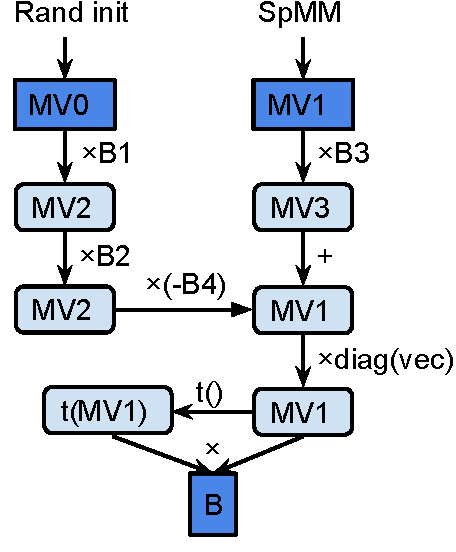
\includegraphics[scale=0.5]{./dag.pdf}
%\vspace{-5pt}
%\caption{A directed acyclic graph represents the sequence of matrix operations
%shown in Figure \ref{comp_seq}. Each rounded rectangular node indicates
%a virtual matrix and each rectangular node indicates a materialized matrix.}
%\vspace{-5pt}
%\label{dag}
%\end{figure}

To perform actual computation, FlashEigen needs to materialize
\textit{virtual matrices}. It materializes a \textit{virtual matrix} when
encountering \textit{op3} and \textit{op6} because these two operations
output Anasazi's native matrices and vectors.
A \textit{virtual matrix} represents some computation on some materialized
tall-and-skinny matrices stored on SSDs. FlashEigen materializes
a \textit{virtual matrix}, which has more than one materialized input matrix,
to minimize the amount of data read from SSDs.
%FlashEigen also materializes all of the dense matrices in the basis.

A \textit{virtual matrix} may contain a sequence of operations, so materializing
it may trigger matrix materialization recursively. We discard the materialized
partition of an intermediate matrix, once it is no longer needed, to avoid
writing data of an intermediate matrix to SSDs.
We partition a \textit{virtual matrix} horizontally in the same fashion as
the external-memory matrices and materialize each partation independantly. 
To increase CPU cache hits, we use a much smaller partition size than
the external-memory matrix. As such, the output of the previous operation is
still in the CPU cache when it is fed to the next operation.

\subsubsection{Matrix caching}
FlashEigen deploys two forms of matrix caching to reduce I/O to SSDs.
In the first case, FlashEigen worker threads cache part of a tall-and-skinny
matrix locally. In the other case, FlashEigen can also cache the most recent
tall-and-skinny matrix in the vector subspace.

Caching part of a tall-and-skinny matrix read from SSDs benefits some of
the matrix operations. One example is the optimization for $op3$ in section
\ref{par_em}, which breaks a large group of dense matrices into multiple
subgroups and the matrix in the right operand is shared by all of the subgroups.
A worker thread only needs to cache data in a row interval of the right matrix
that is currently being processed
because a thread processes one row interval at a time and each row interval of
the tall-and-skinny matrices is processed only once.
Therefore, a worker thread can buffers the data in a row interval of a matrix
locally and accessing the buffered data doesn't incur any locking overhead.

When we buffer the recent portions, we need to give each matrix a data identifier
to identify its data, so we can recognize which portion of data can be reused.
For certain operations, even though a new matrix is created, the data inside
remains the same. A typical example is transpose. The identifier we give to
each matrix should identify the data inside a matrix instead of individual matrices,
so a transposed matrix and its original matrix should share the same identifier.

FlashEigen also caches the most recent tall-and-skinny matrix in the vector
subspace if the RAM of a machine is sufficient to accommodate the entire matrix.
When a new matrix in the vector subspace is generated by sparse matrix
multiplication, an eigensolver needs to perform a sequence of operations on it,
which includes reorgonalization. By caching the matrix in memory, we can
significantly reduce the amount of data written to SSDs.


\section{Experimental Evaluation}

We use a very large SAFS RAID block size. We should mention the sequential I/O performance
of the SSD array.

\subsection{Matrix multiplication}

Matrix multiplication is the most important operation in an eigensolver.
Both sparse matrix multiplication and dense matrix multiplication together
account for most of the computation.

\subsubsection{Sparse matrix dense matrix multiplication}
This section evaluates the performance of the in-memory (mem), semi-external-memory
(SEM) and external-memory (EM) version of SpMM in our eigensolvers. We compares
their performance with that of Intel MKL implementation.
We should vary the number of columns in the dense matrix to show that EM SpMM and SEM SpMM will
eventually catch the performance of in-mem SpMM. Another point is that our SpMM outperforms
Intel MKL.

\dz{I should also plot a chart to show the effectiveness of each optimization
in SpMM.}

\begin{figure}
	\begin{center}
		\footnotesize
		\vspace{-15pt}
		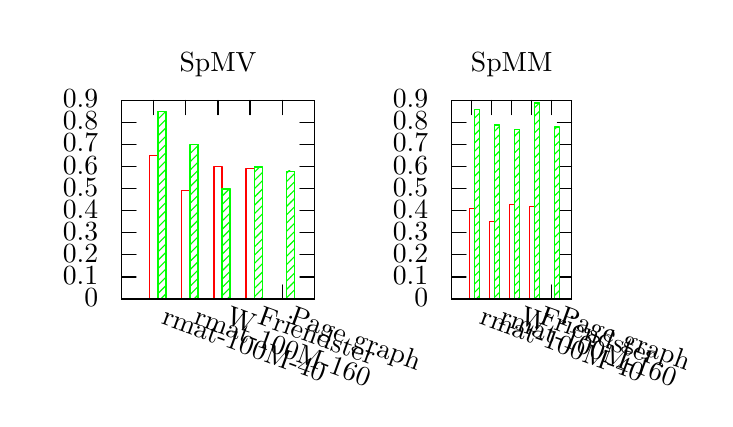
\begin{tikzpicture}[gnuplot]
%% generated with GNUPLOT 4.6p4 (Lua 5.1; terminal rev. 99, script rev. 100)
%% Wed 11 Nov 2015 01:13:24 AM EST
\path (0.000,0.000) rectangle (8.382,4.572);
\gpcolor{color=gp lt color border}
\gpsetlinetype{gp lt border}
\gpsetlinewidth{1.00}
\draw[gp path] (1.196,1.126)--(1.376,1.126);
\draw[gp path] (3.638,1.126)--(3.458,1.126);
\node[gp node right] at (1.012,1.126) { 0};
\draw[gp path] (1.196,1.406)--(1.376,1.406);
\draw[gp path] (3.638,1.406)--(3.458,1.406);
\node[gp node right] at (1.012,1.406) { 0.1};
\draw[gp path] (1.196,1.686)--(1.376,1.686);
\draw[gp path] (3.638,1.686)--(3.458,1.686);
\node[gp node right] at (1.012,1.686) { 0.2};
\draw[gp path] (1.196,1.966)--(1.376,1.966);
\draw[gp path] (3.638,1.966)--(3.458,1.966);
\node[gp node right] at (1.012,1.966) { 0.3};
\draw[gp path] (1.196,2.246)--(1.376,2.246);
\draw[gp path] (3.638,2.246)--(3.458,2.246);
\node[gp node right] at (1.012,2.246) { 0.4};
\draw[gp path] (1.196,2.527)--(1.376,2.527);
\draw[gp path] (3.638,2.527)--(3.458,2.527);
\node[gp node right] at (1.012,2.527) { 0.5};
\draw[gp path] (1.196,2.807)--(1.376,2.807);
\draw[gp path] (3.638,2.807)--(3.458,2.807);
\node[gp node right] at (1.012,2.807) { 0.6};
\draw[gp path] (1.196,3.087)--(1.376,3.087);
\draw[gp path] (3.638,3.087)--(3.458,3.087);
\node[gp node right] at (1.012,3.087) { 0.7};
\draw[gp path] (1.196,3.367)--(1.376,3.367);
\draw[gp path] (3.638,3.367)--(3.458,3.367);
\node[gp node right] at (1.012,3.367) { 0.8};
\draw[gp path] (1.196,3.647)--(1.376,3.647);
\draw[gp path] (3.638,3.647)--(3.458,3.647);
\node[gp node right] at (1.012,3.647) { 0.9};
\draw[gp path] (1.603,1.126)--(1.603,1.306);
\draw[gp path] (1.603,3.647)--(1.603,3.467);
\node[gp node left,rotate=-20] at (1.603,0.942) {rmat-100M-40};
\draw[gp path] (2.010,1.126)--(2.010,1.306);
\draw[gp path] (2.010,3.647)--(2.010,3.467);
\node[gp node left,rotate=-20] at (2.010,0.942) {rmat-100M-160};
\draw[gp path] (2.417,1.126)--(2.417,1.306);
\draw[gp path] (2.417,3.647)--(2.417,3.467);
\node[gp node left,rotate=-20] at (2.417,0.942) {W};
\draw[gp path] (2.824,1.126)--(2.824,1.306);
\draw[gp path] (2.824,3.647)--(2.824,3.467);
\node[gp node left,rotate=-20] at (2.824,0.942) {Friendster};
\draw[gp path] (3.231,1.126)--(3.231,1.306);
\draw[gp path] (3.231,3.647)--(3.231,3.467);
\node[gp node left,rotate=-20] at (3.231,0.942) {Page graph};
\draw[gp path] (1.196,3.647)--(1.196,1.126)--(3.638,1.126)--(3.638,3.647)--cycle;
\node[gp node center] at (2.417,4.109) {SpMV};
\def\gpfillpath{(1.552,1.126)--(1.655,1.126)--(1.655,2.948)--(1.552,2.948)--cycle}
\gpfill{color=gpbgfillcolor} \gpfillpath;
\gpfill{color=gp lt color 0,gp pattern 0,pattern color=.} \gpfillpath;
\gpcolor{color=gp lt color 0}
\gpsetlinetype{gp lt plot 0}
\draw[gp path] (1.552,1.126)--(1.552,2.947)--(1.654,2.947)--(1.654,1.126)--cycle;
\def\gpfillpath{(1.959,1.126)--(2.062,1.126)--(2.062,2.500)--(1.959,2.500)--cycle}
\gpfill{color=gpbgfillcolor} \gpfillpath;
\gpfill{color=gp lt color 0,gp pattern 0,pattern color=.} \gpfillpath;
\draw[gp path] (1.959,1.126)--(1.959,2.499)--(2.061,2.499)--(2.061,1.126)--cycle;
\def\gpfillpath{(2.366,1.126)--(2.469,1.126)--(2.469,2.808)--(2.366,2.808)--cycle}
\gpfill{color=gpbgfillcolor} \gpfillpath;
\gpfill{color=gp lt color 0,gp pattern 0,pattern color=.} \gpfillpath;
\draw[gp path] (2.366,1.126)--(2.366,2.807)--(2.468,2.807)--(2.468,1.126)--cycle;
\def\gpfillpath{(2.773,1.126)--(2.876,1.126)--(2.876,2.780)--(2.773,2.780)--cycle}
\gpfill{color=gpbgfillcolor} \gpfillpath;
\gpfill{color=gp lt color 0,gp pattern 0,pattern color=.} \gpfillpath;
\draw[gp path] (2.773,1.126)--(2.773,2.779)--(2.875,2.779)--(2.875,1.126)--cycle;
\def\gpfillpath{(1.654,1.126)--(1.757,1.126)--(1.757,3.508)--(1.654,3.508)--cycle}
\gpfill{color=gpbgfillcolor} \gpfillpath;
\gpfill{color=gp lt color 1,gp pattern 1,pattern color=.} \gpfillpath;
\gpcolor{color=gp lt color 1}
\gpsetlinetype{gp lt plot 1}
\draw[gp path] (1.654,1.126)--(1.654,3.507)--(1.756,3.507)--(1.756,1.126)--cycle;
\def\gpfillpath{(2.061,1.126)--(2.164,1.126)--(2.164,3.088)--(2.061,3.088)--cycle}
\gpfill{color=gpbgfillcolor} \gpfillpath;
\gpfill{color=gp lt color 1,gp pattern 1,pattern color=.} \gpfillpath;
\draw[gp path] (2.061,1.126)--(2.061,3.087)--(2.163,3.087)--(2.163,1.126)--cycle;
\def\gpfillpath{(2.468,1.126)--(2.571,1.126)--(2.571,2.528)--(2.468,2.528)--cycle}
\gpfill{color=gpbgfillcolor} \gpfillpath;
\gpfill{color=gp lt color 1,gp pattern 1,pattern color=.} \gpfillpath;
\draw[gp path] (2.468,1.126)--(2.468,2.527)--(2.570,2.527)--(2.570,1.126)--cycle;
\def\gpfillpath{(2.875,1.126)--(2.978,1.126)--(2.978,2.808)--(2.875,2.808)--cycle}
\gpfill{color=gpbgfillcolor} \gpfillpath;
\gpfill{color=gp lt color 1,gp pattern 1,pattern color=.} \gpfillpath;
\draw[gp path] (2.875,1.126)--(2.875,2.807)--(2.977,2.807)--(2.977,1.126)--cycle;
\def\gpfillpath{(3.282,1.126)--(3.385,1.126)--(3.385,2.752)--(3.282,2.752)--cycle}
\gpfill{color=gpbgfillcolor} \gpfillpath;
\gpfill{color=gp lt color 1,gp pattern 1,pattern color=.} \gpfillpath;
\draw[gp path] (3.282,1.126)--(3.282,2.751)--(3.384,2.751)--(3.384,1.126)--cycle;
\gpcolor{color=gp lt color border}
\gpsetlinetype{gp lt border}
\draw[gp path] (1.196,3.647)--(1.196,1.126)--(3.638,1.126)--(3.638,3.647)--cycle;
%% coordinates of the plot area
\gpdefrectangularnode{gp plot 1}{\pgfpoint{1.196cm}{1.126cm}}{\pgfpoint{3.638cm}{3.647cm}}
\draw[gp path] (5.387,1.126)--(5.567,1.126);
\draw[gp path] (6.907,1.126)--(6.727,1.126);
\node[gp node right] at (5.203,1.126) { 0};
\draw[gp path] (5.387,1.406)--(5.567,1.406);
\draw[gp path] (6.907,1.406)--(6.727,1.406);
\node[gp node right] at (5.203,1.406) { 0.1};
\draw[gp path] (5.387,1.686)--(5.567,1.686);
\draw[gp path] (6.907,1.686)--(6.727,1.686);
\node[gp node right] at (5.203,1.686) { 0.2};
\draw[gp path] (5.387,1.966)--(5.567,1.966);
\draw[gp path] (6.907,1.966)--(6.727,1.966);
\node[gp node right] at (5.203,1.966) { 0.3};
\draw[gp path] (5.387,2.246)--(5.567,2.246);
\draw[gp path] (6.907,2.246)--(6.727,2.246);
\node[gp node right] at (5.203,2.246) { 0.4};
\draw[gp path] (5.387,2.527)--(5.567,2.527);
\draw[gp path] (6.907,2.527)--(6.727,2.527);
\node[gp node right] at (5.203,2.527) { 0.5};
\draw[gp path] (5.387,2.807)--(5.567,2.807);
\draw[gp path] (6.907,2.807)--(6.727,2.807);
\node[gp node right] at (5.203,2.807) { 0.6};
\draw[gp path] (5.387,3.087)--(5.567,3.087);
\draw[gp path] (6.907,3.087)--(6.727,3.087);
\node[gp node right] at (5.203,3.087) { 0.7};
\draw[gp path] (5.387,3.367)--(5.567,3.367);
\draw[gp path] (6.907,3.367)--(6.727,3.367);
\node[gp node right] at (5.203,3.367) { 0.8};
\draw[gp path] (5.387,3.647)--(5.567,3.647);
\draw[gp path] (6.907,3.647)--(6.727,3.647);
\node[gp node right] at (5.203,3.647) { 0.9};
\draw[gp path] (5.640,1.126)--(5.640,1.306);
\draw[gp path] (5.640,3.647)--(5.640,3.467);
\node[gp node left,rotate=-20] at (5.640,0.942) {rmat-100M-40};
\draw[gp path] (5.894,1.126)--(5.894,1.306);
\draw[gp path] (5.894,3.647)--(5.894,3.467);
\node[gp node left,rotate=-20] at (5.894,0.942) {rmat-100M-160};
\draw[gp path] (6.147,1.126)--(6.147,1.306);
\draw[gp path] (6.147,3.647)--(6.147,3.467);
\node[gp node left,rotate=-20] at (6.147,0.942) {W};
\draw[gp path] (6.400,1.126)--(6.400,1.306);
\draw[gp path] (6.400,3.647)--(6.400,3.467);
\node[gp node left,rotate=-20] at (6.400,0.942) {Friendster};
\draw[gp path] (6.654,1.126)--(6.654,1.306);
\draw[gp path] (6.654,3.647)--(6.654,3.467);
\node[gp node left,rotate=-20] at (6.654,0.942) {Page graph};
\draw[gp path] (5.387,3.647)--(5.387,1.126)--(6.907,1.126)--(6.907,3.647)--cycle;
\node[gp node center] at (6.147,4.109) {SpMM};
\def\gpfillpath{(5.609,1.126)--(5.673,1.126)--(5.673,2.275)--(5.609,2.275)--cycle}
\gpfill{color=gpbgfillcolor} \gpfillpath;
\gpfill{color=gp lt color 0,gp pattern 0,pattern color=.} \gpfillpath;
\gpcolor{color=gp lt color 0}
\gpsetlinetype{gp lt plot 0}
\draw[gp path] (5.609,1.126)--(5.609,2.274)--(5.672,2.274)--(5.672,1.126)--cycle;
\def\gpfillpath{(5.862,1.126)--(5.926,1.126)--(5.926,2.107)--(5.862,2.107)--cycle}
\gpfill{color=gpbgfillcolor} \gpfillpath;
\gpfill{color=gp lt color 0,gp pattern 0,pattern color=.} \gpfillpath;
\draw[gp path] (5.862,1.126)--(5.862,2.106)--(5.925,2.106)--(5.925,1.126)--cycle;
\def\gpfillpath{(6.115,1.126)--(6.180,1.126)--(6.180,2.331)--(6.115,2.331)--cycle}
\gpfill{color=gpbgfillcolor} \gpfillpath;
\gpfill{color=gp lt color 0,gp pattern 0,pattern color=.} \gpfillpath;
\draw[gp path] (6.115,1.126)--(6.115,2.330)--(6.179,2.330)--(6.179,1.126)--cycle;
\def\gpfillpath{(6.369,1.126)--(6.433,1.126)--(6.433,2.303)--(6.369,2.303)--cycle}
\gpfill{color=gpbgfillcolor} \gpfillpath;
\gpfill{color=gp lt color 0,gp pattern 0,pattern color=.} \gpfillpath;
\draw[gp path] (6.369,1.126)--(6.369,2.302)--(6.432,2.302)--(6.432,1.126)--cycle;
\def\gpfillpath{(5.672,1.126)--(5.736,1.126)--(5.736,3.536)--(5.672,3.536)--cycle}
\gpfill{color=gpbgfillcolor} \gpfillpath;
\gpfill{color=gp lt color 1,gp pattern 1,pattern color=.} \gpfillpath;
\gpcolor{color=gp lt color 1}
\gpsetlinetype{gp lt plot 1}
\draw[gp path] (5.672,1.126)--(5.672,3.535)--(5.735,3.535)--(5.735,1.126)--cycle;
\def\gpfillpath{(5.925,1.126)--(5.990,1.126)--(5.990,3.340)--(5.925,3.340)--cycle}
\gpfill{color=gpbgfillcolor} \gpfillpath;
\gpfill{color=gp lt color 1,gp pattern 1,pattern color=.} \gpfillpath;
\draw[gp path] (5.925,1.126)--(5.925,3.339)--(5.989,3.339)--(5.989,1.126)--cycle;
\def\gpfillpath{(6.179,1.126)--(6.243,1.126)--(6.243,3.284)--(6.179,3.284)--cycle}
\gpfill{color=gpbgfillcolor} \gpfillpath;
\gpfill{color=gp lt color 1,gp pattern 1,pattern color=.} \gpfillpath;
\draw[gp path] (6.179,1.126)--(6.179,3.283)--(6.242,3.283)--(6.242,1.126)--cycle;
\def\gpfillpath{(6.432,1.126)--(6.496,1.126)--(6.496,3.620)--(6.432,3.620)--cycle}
\gpfill{color=gpbgfillcolor} \gpfillpath;
\gpfill{color=gp lt color 1,gp pattern 1,pattern color=.} \gpfillpath;
\draw[gp path] (6.432,1.126)--(6.432,3.619)--(6.495,3.619)--(6.495,1.126)--cycle;
\def\gpfillpath{(6.685,1.126)--(6.750,1.126)--(6.750,3.312)--(6.685,3.312)--cycle}
\gpfill{color=gpbgfillcolor} \gpfillpath;
\gpfill{color=gp lt color 1,gp pattern 1,pattern color=.} \gpfillpath;
\draw[gp path] (6.685,1.126)--(6.685,3.311)--(6.749,3.311)--(6.749,1.126)--cycle;
\gpcolor{color=gp lt color border}
\gpsetlinetype{gp lt border}
\draw[gp path] (5.387,3.647)--(5.387,1.126)--(6.907,1.126)--(6.907,3.647)--cycle;
%% coordinates of the plot area
\gpdefrectangularnode{gp plot 2}{\pgfpoint{5.387cm}{1.126cm}}{\pgfpoint{6.907cm}{3.647cm}}
\end{tikzpicture}
%% gnuplot variables

		\vspace{-15pt}
		\caption{The performance of the in-memory, SEM and EM implementations
			of SpMM in our eigensolvers on the Friendster graph. The performance
			is normalized to the Intel MKL. \dz{measure the SEM performance.}}
		\label{perf:spmm}
	\end{center}
\end{figure}

One of the reason that MKL is slow is that MKL cannot balance the load well.

\begin{figure}
	\begin{center}
		\footnotesize
		\vspace{-15pt}
		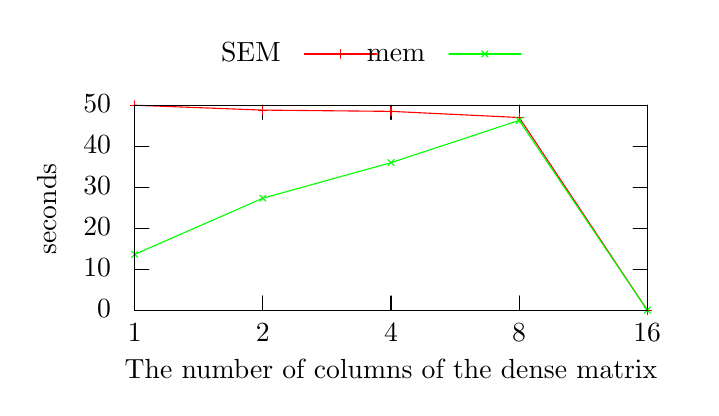
\begin{tikzpicture}[gnuplot]
%% generated with GNUPLOT 4.6p4 (Lua 5.1; terminal rev. 99, script rev. 100)
%% Wed 22 Jul 2015 12:34:54 AM EDT
\path (0.000,0.000) rectangle (8.382,4.572);
\gpcolor{color=gp lt color border}
\gpsetlinetype{gp lt border}
\gpsetlinewidth{1.00}
\draw[gp path] (1.320,0.985)--(1.500,0.985);
\draw[gp path] (7.829,0.985)--(7.649,0.985);
\node[gp node right] at (1.136,0.985) { 0};
\draw[gp path] (1.320,1.505)--(1.500,1.505);
\draw[gp path] (7.829,1.505)--(7.649,1.505);
\node[gp node right] at (1.136,1.505) { 10};
\draw[gp path] (1.320,2.026)--(1.500,2.026);
\draw[gp path] (7.829,2.026)--(7.649,2.026);
\node[gp node right] at (1.136,2.026) { 20};
\draw[gp path] (1.320,2.546)--(1.500,2.546);
\draw[gp path] (7.829,2.546)--(7.649,2.546);
\node[gp node right] at (1.136,2.546) { 30};
\draw[gp path] (1.320,3.067)--(1.500,3.067);
\draw[gp path] (7.829,3.067)--(7.649,3.067);
\node[gp node right] at (1.136,3.067) { 40};
\draw[gp path] (1.320,3.587)--(1.500,3.587);
\draw[gp path] (7.829,3.587)--(7.649,3.587);
\node[gp node right] at (1.136,3.587) { 50};
\draw[gp path] (1.320,0.985)--(1.320,1.165);
\draw[gp path] (1.320,3.587)--(1.320,3.407);
\node[gp node center] at (1.320,0.677) {1};
\draw[gp path] (2.947,0.985)--(2.947,1.165);
\draw[gp path] (2.947,3.587)--(2.947,3.407);
\node[gp node center] at (2.947,0.677) {2};
\draw[gp path] (4.575,0.985)--(4.575,1.165);
\draw[gp path] (4.575,3.587)--(4.575,3.407);
\node[gp node center] at (4.575,0.677) {4};
\draw[gp path] (6.202,0.985)--(6.202,1.165);
\draw[gp path] (6.202,3.587)--(6.202,3.407);
\node[gp node center] at (6.202,0.677) {8};
\draw[gp path] (7.829,0.985)--(7.829,1.165);
\draw[gp path] (7.829,3.587)--(7.829,3.407);
\node[gp node center] at (7.829,0.677) {16};
\draw[gp path] (1.320,3.587)--(1.320,0.985)--(7.829,0.985)--(7.829,3.587)--cycle;
\node[gp node center,rotate=-270] at (0.246,2.286) {seconds};
\node[gp node center] at (4.574,0.215) {The number of columns of the dense matrix};
\node[gp node right] at (3.290,4.238) {SEM};
\gpcolor{color=gp lt color 0}
\gpsetlinetype{gp lt plot 0}
\draw[gp path] (3.474,4.238)--(4.390,4.238);
\draw[gp path] (1.320,3.587)--(2.947,3.525)--(4.575,3.509)--(6.202,3.431)--(7.829,0.985);
\gpsetpointsize{4.00}
\gppoint{gp mark 1}{(1.320,3.587)}
\gppoint{gp mark 1}{(2.947,3.525)}
\gppoint{gp mark 1}{(4.575,3.509)}
\gppoint{gp mark 1}{(6.202,3.431)}
\gppoint{gp mark 1}{(7.829,0.985)}
\gppoint{gp mark 1}{(3.932,4.238)}
\gpcolor{color=gp lt color border}
\node[gp node right] at (5.126,4.238) {mem};
\gpcolor{color=gp lt color 1}
\gpsetlinetype{gp lt plot 1}
\draw[gp path] (5.310,4.238)--(6.226,4.238);
\draw[gp path] (1.320,1.693)--(2.947,2.406)--(4.575,2.858)--(6.202,3.394)--(7.829,0.985);
\gppoint{gp mark 2}{(1.320,1.693)}
\gppoint{gp mark 2}{(2.947,2.406)}
\gppoint{gp mark 2}{(4.575,2.858)}
\gppoint{gp mark 2}{(6.202,3.394)}
\gppoint{gp mark 2}{(7.829,0.985)}
\gppoint{gp mark 2}{(5.768,4.238)}
\gpcolor{color=gp lt color border}
\gpsetlinetype{gp lt border}
\draw[gp path] (1.320,3.587)--(1.320,0.985)--(7.829,0.985)--(7.829,3.587)--cycle;
%% coordinates of the plot area
\gpdefrectangularnode{gp plot 1}{\pgfpoint{1.320cm}{0.985cm}}{\pgfpoint{7.829cm}{3.587cm}}
\end{tikzpicture}
%% gnuplot variables

		\vspace{-15pt}
		\caption{The performance of the in-memory, SEM and EM version of SpMM
			in our eigensolvers on the page graph.}
		\label{perf:spmm_pg}
	\end{center}
\end{figure}

\subsubsection{Dense matrix multiplication}

Figure \ref{perf:mat_mul} shows the relative performance of the in-memory
and external memory version of dense matrix multiplication.
There is a large gap between in-memory and external-memory implementation.
The SSDs are the bottleneck. This is not surprising because the sequential
I/O performance of SSDs is an order of magnitude smaller than RAM.
However, this indicates that we can use the extra computation to save I/O.
When the number of columns in the dense matrices increase, the performance
gap gets smaller, which indicates that when computing more eigenpairs,
the performance gap between in-memory and external-memory eigensolvers
will be smaller.

\begin{figure}
	\begin{center}
		\footnotesize
		\vspace{-15pt}
		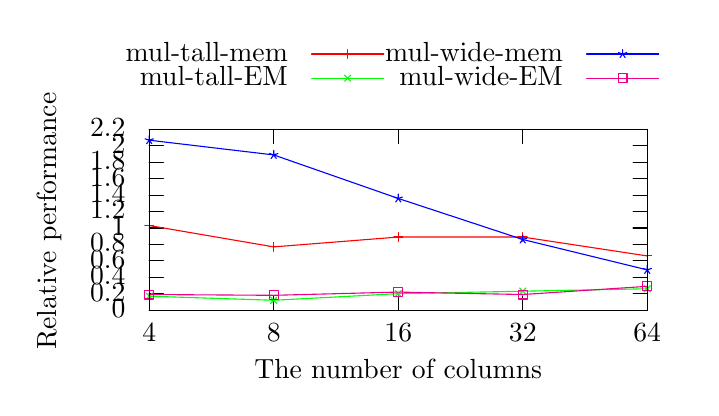
\begin{tikzpicture}[gnuplot]
%% generated with GNUPLOT 4.6p4 (Lua 5.1; terminal rev. 99, script rev. 100)
%% Wed 22 Jul 2015 04:02:11 PM EDT
\path (0.000,0.000) rectangle (8.382,4.572);
\gpcolor{color=gp lt color border}
\gpsetlinetype{gp lt border}
\gpsetlinewidth{1.00}
\draw[gp path] (1.504,0.985)--(1.684,0.985);
\draw[gp path] (7.829,0.985)--(7.649,0.985);
\node[gp node right] at (1.320,0.985) { 0};
\draw[gp path] (1.504,1.194)--(1.684,1.194);
\draw[gp path] (7.829,1.194)--(7.649,1.194);
\node[gp node right] at (1.320,1.194) { 0.2};
\draw[gp path] (1.504,1.402)--(1.684,1.402);
\draw[gp path] (7.829,1.402)--(7.649,1.402);
\node[gp node right] at (1.320,1.402) { 0.4};
\draw[gp path] (1.504,1.611)--(1.684,1.611);
\draw[gp path] (7.829,1.611)--(7.649,1.611);
\node[gp node right] at (1.320,1.611) { 0.6};
\draw[gp path] (1.504,1.819)--(1.684,1.819);
\draw[gp path] (7.829,1.819)--(7.649,1.819);
\node[gp node right] at (1.320,1.819) { 0.8};
\draw[gp path] (1.504,2.028)--(1.684,2.028);
\draw[gp path] (7.829,2.028)--(7.649,2.028);
\node[gp node right] at (1.320,2.028) { 1};
\draw[gp path] (1.504,2.236)--(1.684,2.236);
\draw[gp path] (7.829,2.236)--(7.649,2.236);
\node[gp node right] at (1.320,2.236) { 1.2};
\draw[gp path] (1.504,2.445)--(1.684,2.445);
\draw[gp path] (7.829,2.445)--(7.649,2.445);
\node[gp node right] at (1.320,2.445) { 1.4};
\draw[gp path] (1.504,2.653)--(1.684,2.653);
\draw[gp path] (7.829,2.653)--(7.649,2.653);
\node[gp node right] at (1.320,2.653) { 1.6};
\draw[gp path] (1.504,2.862)--(1.684,2.862);
\draw[gp path] (7.829,2.862)--(7.649,2.862);
\node[gp node right] at (1.320,2.862) { 1.8};
\draw[gp path] (1.504,3.070)--(1.684,3.070);
\draw[gp path] (7.829,3.070)--(7.649,3.070);
\node[gp node right] at (1.320,3.070) { 2};
\draw[gp path] (1.504,3.279)--(1.684,3.279);
\draw[gp path] (7.829,3.279)--(7.649,3.279);
\node[gp node right] at (1.320,3.279) { 2.2};
\draw[gp path] (1.504,0.985)--(1.504,1.165);
\draw[gp path] (1.504,3.279)--(1.504,3.099);
\node[gp node center] at (1.504,0.677) {4};
\draw[gp path] (3.085,0.985)--(3.085,1.165);
\draw[gp path] (3.085,3.279)--(3.085,3.099);
\node[gp node center] at (3.085,0.677) {8};
\draw[gp path] (4.667,0.985)--(4.667,1.165);
\draw[gp path] (4.667,3.279)--(4.667,3.099);
\node[gp node center] at (4.667,0.677) {16};
\draw[gp path] (6.248,0.985)--(6.248,1.165);
\draw[gp path] (6.248,3.279)--(6.248,3.099);
\node[gp node center] at (6.248,0.677) {32};
\draw[gp path] (7.829,0.985)--(7.829,1.165);
\draw[gp path] (7.829,3.279)--(7.829,3.099);
\node[gp node center] at (7.829,0.677) {64};
\draw[gp path] (1.504,3.279)--(1.504,0.985)--(7.829,0.985)--(7.829,3.279)--cycle;
\node[gp node center,rotate=-270] at (0.246,2.132) {Relative performance};
\node[gp node center] at (4.666,0.215) {The number of columns};
\node[gp node right] at (3.382,4.238) {mul-tall-mem};
\gpcolor{color=gp lt color 0}
\gpsetlinetype{gp lt plot 0}
\draw[gp path] (3.566,4.238)--(4.482,4.238);
\draw[gp path] (1.504,2.059)--(3.085,1.788)--(4.667,1.913)--(6.248,1.913)--(7.829,1.673);
\gpsetpointsize{4.00}
\gppoint{gp mark 1}{(1.504,2.059)}
\gppoint{gp mark 1}{(3.085,1.788)}
\gppoint{gp mark 1}{(4.667,1.913)}
\gppoint{gp mark 1}{(6.248,1.913)}
\gppoint{gp mark 1}{(7.829,1.673)}
\gppoint{gp mark 1}{(4.024,4.238)}
\gpcolor{color=gp lt color border}
\node[gp node right] at (3.382,3.930) {mul-tall-EM};
\gpcolor{color=gp lt color 1}
\gpsetlinetype{gp lt plot 1}
\draw[gp path] (3.566,3.930)--(4.482,3.930);
\draw[gp path] (1.504,1.162)--(3.085,1.110)--(4.667,1.194)--(6.248,1.225)--(7.829,1.256);
\gppoint{gp mark 2}{(1.504,1.162)}
\gppoint{gp mark 2}{(3.085,1.110)}
\gppoint{gp mark 2}{(4.667,1.194)}
\gppoint{gp mark 2}{(6.248,1.225)}
\gppoint{gp mark 2}{(7.829,1.256)}
\gppoint{gp mark 2}{(4.024,3.930)}
\gpcolor{color=gp lt color border}
\node[gp node right] at (6.874,4.238) {mul-wide-mem};
\gpcolor{color=gp lt color 2}
\gpsetlinetype{gp lt plot 2}
\draw[gp path] (7.058,4.238)--(7.974,4.238);
\draw[gp path] (1.504,3.143)--(3.085,2.956)--(4.667,2.403)--(6.248,1.882)--(7.829,1.496);
\gppoint{gp mark 3}{(1.504,3.143)}
\gppoint{gp mark 3}{(3.085,2.956)}
\gppoint{gp mark 3}{(4.667,2.403)}
\gppoint{gp mark 3}{(6.248,1.882)}
\gppoint{gp mark 3}{(7.829,1.496)}
\gppoint{gp mark 3}{(7.516,4.238)}
\gpcolor{color=gp lt color border}
\node[gp node right] at (6.874,3.930) {mul-wide-EM};
\gpcolor{color=gp lt color 3}
\gpsetlinetype{gp lt plot 3}
\draw[gp path] (7.058,3.930)--(7.974,3.930);
\draw[gp path] (1.504,1.183)--(3.085,1.173)--(4.667,1.214)--(6.248,1.183)--(7.829,1.287);
\gppoint{gp mark 4}{(1.504,1.183)}
\gppoint{gp mark 4}{(3.085,1.173)}
\gppoint{gp mark 4}{(4.667,1.214)}
\gppoint{gp mark 4}{(6.248,1.183)}
\gppoint{gp mark 4}{(7.829,1.287)}
\gppoint{gp mark 4}{(7.516,3.930)}
\gpcolor{color=gp lt color border}
\gpsetlinetype{gp lt border}
\draw[gp path] (1.504,3.279)--(1.504,0.985)--(7.829,0.985)--(7.829,3.279)--cycle;
%% coordinates of the plot area
\gpdefrectangularnode{gp plot 1}{\pgfpoint{1.504cm}{0.985cm}}{\pgfpoint{7.829cm}{3.279cm}}
\end{tikzpicture}
%% gnuplot variables

		\vspace{-15pt}
		\caption{The performance of in-memory and EM implementations of two types
			of matrix multiplication: a tall matrix ($200M \times X$) times
			a small matrix ($X \times X$) and a wide matrix ($X \times 200M$)
			times a tall matrix ($200M \times X$). Their performance is
		normalized by the corresponding Intel MKL implementations.}
		\label{perf:mat_mul}
	\end{center}
\end{figure}

\dz{Further optimize the in-memory dense matrix multiplication.}

\subsection{Lazy evaluation}
How effective are the optimizations for a group of dense matrix operations?

In this section, we evaluate how aggressively we should materialize virtual
matrices. What is the sweet spot that balance computation and I/O.

We should plot a chart with multiple lines:
in-mem version with all matrices materialized,
in-mem version with matrices lazily evaluated,
EM version with all matrices materialized,
EM version with matrices lazily evaluated.

In this chart, we only count the time used by dense matrix operations.

\subsection{Compare EM eigensolvers with in-memory eigensolvers}
We compare our EM eigensolvers with our in-mem eigensolvers as well as the original
Anasazi eigensolvers. For the in-mem eigensolver, it should also have two versions.
One version is to materialize all dense matrix operations and the other version is
to materialize virtual matrices in the same approach as the EM eigensolvers.

\subsubsection{Tuning the eigensolver for faster convergence}
We need to trade off memory/disk space with speed and the number of writes.
The larger column matrix we store, the fewer iterations are required. However,
it is unclear how a large column matrix affects the amount of data written disks.
If we implement dense matrix operations naively, a large column matrix helps to
reduce the amount of data written to disks; if we avoid materializing a dense
matrix every time we generate a dense matrix, a smaller column matrix potentially
reduce the amount of data written to disks.

\begin{table}
	\begin{center}
		\small
		\begin{tabular}{|c|c|c|c|c|}
			\hline
			eigensolver & block size & the number of blocks \\
			\hline
			Krylov-Schur & 4 & \# eigenpairs \\
			\hline
			Davidson & \# eigenpairs & 8 \\
			\hline
			LOBPCG &  & N/A \\
			\hline
		\end{tabular}
		\normalsize
	\end{center}
	\caption{}
	\label{eigen_conf}
\end{table}

The block eigensolvers have two parameters that significantly affect
the convergence rate. One is the block size, which determines the number
of vectors in the subspace that operate together. The other is the number
of blocks. Table \ref{eigen_conf} summaries the configuration that performs
well in general for different numbers of eigenpairs and different eigenvalue
problems. The LOBPCG eigensolver is the special case that only allows users
to specify the block size.

The computation complexity increases roughly linearly with the number of blocks
and the square of the block size.

\subsubsection{Performance of eigensolvers}

When computing hundreds of eigenpairs, an EM eigensolver may be able to outperform
an in-mem version.

To compute hundreds of eigenpairs, we need a large block size, which means
the dense matrix has a large number of columns. EM multiplication of such
a large matrix has performance similar to in-mem version. Furthermore,
to compute such a large number of eigenpairs, we need a lot of memory to
store the vectors in the basis. The EM eigensolver can store more vectors
for the basis and thus has a faster convergance rate.

We need to show how much read and write we save with lazy evaluation. We should
also show how much multiplication the lazy evaluation causes.


\section{Conclusions}
We present an external-memory framework called FlashEigen using a large array
of commodity SSDs to solve eigenvalue problems at the billion scale. FlashEigen
utilizes the Anasazi framework to get state-of-art eigensolver implementations
so that we can focus on optimizations on sparse matrix multiplication and dense
matrix multiplication on SSDs.

We implement a sparse matrix dense matrix multiplication in the semi-external
memory fashion. That is, we keep the sparse matrix on SSDs and the dense matrices
in memory. We deploy a set of memory and I/O optimizations so that the sparse
matrix dense matrix multiplication has performance comparable to its in-memory
counterparts while significantly outperforming the MKL and Trilinos implementation.
The semi-external sparse matrix multiplication is able to saturate either CPU or
SSDs or both, which suggests that we have achieved the maximal performance from
the existing hardware.

We further implement and optimize external-memory matrix multiplication for
FlashEigen. When computing eigenvalues on many real-world graphs, the storage
size required by the subspace in an eigensolver is massive. Therefore, we keep
the subspace on the SSD array and deploy a set of I/O optimizations on dense
matrix multiplication. With the I/O optimizations, we saturate the SSDs in
dense matrix multiplication and achieve the maximal performance from the existing
hardware. However, the SSD array is an order of magnitude slower than RAM, so
external-memory dense matrix multiplication is about three or four times slower
than the state-of-art in-memory dense matrix multiplication.

We implement our external-memory eigensolver with the semi-external memory
sparse matrix multiplication and the external-memory dense matrix multiplication.
Our experiments show that our external-memory eigensolver achieves at least
30\% of the performance of its in-memory counterparts. For a small number of
eigenvalues, which is the most common case for spectral analysis, our external-memory
eigensolver has less than 50\% performance loss. We further show that our external-
memory eigensolver is able to scale a graph with 3.4 billion vertices and 129
billion edges. It finishes eigendecomposition within a reasonable amount of time
and consumes a fairly small amount of resources. This suggests that our external-
memory eigensolver is able to scale to even a larger eigenvalue problem in our
1TB-RAM machine.

We are able to scale to much larger graphs.
Given the same amount of resources, SSDs significantly extends the memory capacity
and give users the freedom of choosing the optimal subspace size for better convergence.
Our solution also works better for relatively denser graphs.
Our solution works better for computing a small number of eigenvalues.


%\section{Acknowledgments}


{\footnotesize \bibliographystyle{acm}
\bibliography{eigensolver}  % sigproc.bib is the name of the Bibliography in this case


%\theendnotes

\end{document}
